% LetzCV-sleek 1.0 LaTeX template
% Author: Andreï V. Kostyrka, University of Luxembourg
%
% This template fills the gap in the available variety of templates
% by proposing something that is not a custom class, not using any
% hard-coded settings deeply hidden in style files, and provides
% a handful of custom command definitions that are as transparent as it gets.
% Developed at the University of Luxembourg.
%
% Target audience: applicants in the IT industry, or business in general
%
% The main strength of this template is, it explicitly showcases how
% to break the flow of text to achieve the most flexible right alignment
% of dates for multiple configurations.
%
% Modified by Lorenzo Rossi to better suit my needs.

\documentclass[11pt, a4paper]{article}

\usepackage[T1]{fontenc}     % We are using pdfLaTeX,
\usepackage[utf8]{inputenc}  % hence this preparation
\usepackage[british]{babel}
\usepackage[left=0mm, right=0mm, top=0mm, bottom=0mm]{geometry}
\usepackage[stretch=25, shrink=25]{microtype}
\usepackage[none]{hyphenat}  % no hyphenation
\usepackage{graphicx}        % To insert pictures
\usepackage{xcolor}          % To add colour to the document
\usepackage{marvosym}        % Provides icons for the contact details
\usepackage{enumitem}        % To redefine spacing in lists
\usepackage{amssymb}         % For black triangle right
\setlist{parsep=0pt, topsep=0pt, partopsep=1pt, itemsep=1pt, leftmargin=6mm, noitemsep}

\usepackage{FiraSans}        % Font for the document
\renewcommand{\familydefault}{\sfdefault}


% Custom colours
\definecolor{cvblue}{HTML}{49789c}
\definecolor{cvtopic}{HTML}{454545}
\definecolor{cvbullet}{HTML}{373737}

% Custom Bullet
\newcommand{\sbullet}[1][.5]{\textcolor{cvbullet}{\(\mathbin{\vcenter{\hbox{\scalebox{#1}{\(\bullet\)}}}}\)}\hspace{0.5ex}}
\newcommand{\striangle}[1][.5]{\textcolor{cvbullet}{\(\mathbin{\vcenter{\hbox{\scalebox{#1}{\(\blacktriangleright\)}}}}\)}\hspace{0.5ex}}

\newcommand{\bigbullet}{\sbullet[0.65]}
\newcommand{\bigtriangle}{\striangle[0.65]}

% User-defined commands
\newcommand{\dates}[1]{\hfill\mbox{\textbf{#1}}} % Bold stuff that doesn’t got broken into lines
\newcommand{\itemspacing}{\par\vskip 0.25ex} % Item spacing
\newcommand{\leftsection}[1]{\vspace*{2ex}\textsc{\textbf{#1}}\par%
\vspace*{-1.5ex}\hrulefill\par\vspace*{0.7ex}}
\newcommand{\leftsubsection}[1]{\small{#1}}

\newcommand{\sectiontitle}[1]{\vspace*{2.5ex}\textsc{\Large\color{cvblue}#1}\par%
     \vspace*{-2ex}{\color{cvblue}\hrulefill}\par}
\newcommand{\subsectiontitle}[1]{\textbf{\textsc{#1}}}
\newcommand{\nametitle}[1]{\textbf{\Huge\textcolor{cvblue}{#1}}}

% Icons commands
\newcommand{\websiteline}{\par{
\includegraphics[height=10pt]{icons/website_white.png}}\ \href{https://www.lorenzoros.si}{lorenzoros.si}}
\newcommand{\emailline}{\par{
\includegraphics[height=10pt]{icons/email_white.png}}\ \href{mailto:jobs@lorenzoros.si}{jobs@lorenzoros.si} }
\newcommand{\githubline}{\par{
\includegraphics[height=10pt]{icons/github_white.png}}\ \href{https://www.github.com/lorossi}{github.com/lorossi}}
\newcommand{\linkedinline}{\par{
\includegraphics[height=10pt]{icons/linkedin_white.png}}\ \href{https://www.linkedin.com/in/lorenzo-rossi-897628212/}{Lorenzo Rossi}}
\newcommand{\instagramline}{\par{
\includegraphics[height=10pt]{icons/instagram_white.png}}\ \href{https://www.instagram.com/lorossi/}{lorossi}}

\newcommand{\phoneline}{\par{
\includegraphics[height=10pt]{icons/phone_white.png}}\ +39\,331\,102\,4623}
\newcommand{\mapline}{\par{
\includegraphics[height=10pt]{icons/map_white.png}}\ Milano, Italy}

% Custom commands
\newcommand{\topics}[1]{\textcolor{cvtopic}{\small\hfill\textsc{#1}}}
\newcommand{\descript}[1]{\textcolor{black}{\bigbullet\small #1}}


\usepackage[colorlinks = true, urlcolor = white, linkcolor = white]{hyperref}

\begin{document}

% Style definitions -- killing the unnecessary space and adding the skips explicitly
\setlength{\topskip}{0pt}
\setlength{\parindent}{0pt}
\setlength{\parskip}{0pt}
\setlength{\fboxsep}{0pt}
\pagestyle{empty}
\raggedbottom

\begin{minipage}[t]{0.30\textwidth} %% Left column -- outer definition
  %  Left column -- top dark rectangle

  \colorbox{cvblue}{
    \color{white}  %% LEFT BOX
    \hspace{1em}  %% Left margin
    \begin{minipage}[t][\textheight][t]{0.82\textwidth}
      \raggedright
      \vspace*{2.5ex}

      % Centering without extra vertical spacing
      \null\hfill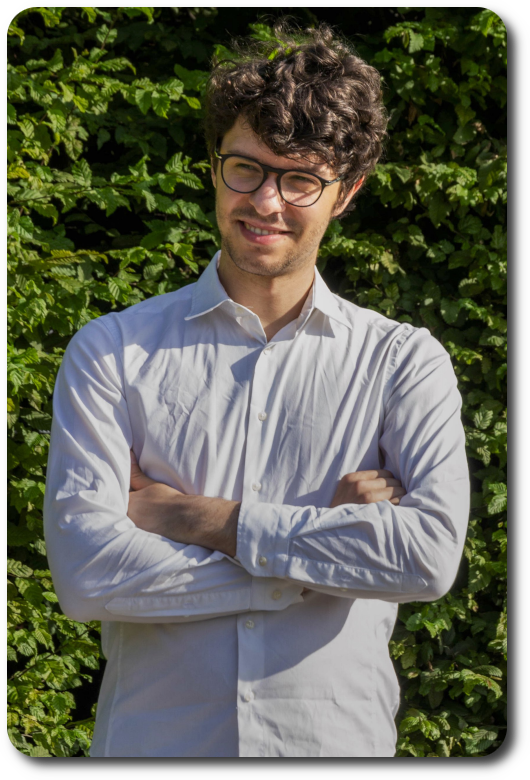
\includegraphics[width=0.75\textwidth]{images/photo.png}\hfill\null

      \vspace*{0.5ex} % Extra space after the picture

      \leftsection{About Me}
      Computer Science and Engineering student. \\
      Technology and programming enthusiast. \\
      Creative project developer. \\

      \leftsection{Contact details}
      \small
      \websiteline \\[0.4ex]
      \githubline \\[0.4ex]
      \instagramline \\[0.4ex]
      \linkedinline
      \emailline \\[0.4ex]
      \phoneline \\[0.4ex]
      \mapline

      \normalsize

      \leftsection{Personal information}
      Birth Date: \textbf{01/02/1997} \\[0.5ex]
      Citizenship: \textbf{Italian} \\[0.5ex]
      Languages:
      \textbf{English} (C1)
      \textbf{French} (B1)
      \textbf{Italian} (native)

      \leftsection{Programming Languages}
      \textbf{Proficient}: C, GDscript, Go, JavaScript, Processing, Python \\
      \textbf{Experienced}: Assembly, Bash, Erlang, Haskell, Java, SQL, Scheme, VHDL \\
      \textbf{Familiar}: C++, Matlab, Rust

      \leftsection{Descriptive Languages}
      CSS, HTML5, LaTeX

      \leftsection{Frameworks}
      Bootstrap, Django, FastAPI, Flask, JQuery, Keras, OpenCV, TensorFlow

      \leftsection{Hobbies}
      Photography, Photo Editing, Digital Art, Cooking, Movie Watching

    \end{minipage}%

    \hspace{1em}  %% Right margin
  }
\end{minipage}% Right column
\hskip2.5em% Left margin for the white area
\begin{minipage}[t]{0.60\textwidth}
  \setlength{\parskip}{0.8ex}% Adds spaces between paragraphs; use \\ to add new lines without this space. Shrink this amount to fit more data vertically

  \vspace{2ex}

  \nametitle{Lorenzo Rossi}

  \sectiontitle{Experience}

  \subsectiontitle{Freelancing} on web platforms
  \dates{October 2020 - Current} \\
  \descript{Areas of expertise: Web Development \textit{(front-end and back-end)}, Embedded Systems, Software Development.} \\
  \descript{Engaged and completed multiple projects involving both embedded \textit{(using ESP32, Arduino and RaspberryPi)} and desktop \textit{(on both Linux and Windows)} systems.} \\
  \descript{Gained important soft skills like dealing with a vast amount of work and collaborating with people all over the world.} \\
  \descript{Got the chance to interface with the real world outside my university and interact with real life projects.}

  \itemspacing

  \sectiontitle{Personal Projects}

  \subsectiontitle{Embedded developer}
  \topics{Arduino | ESP32 | ESP8266 | PIC} \\
  \descript{Experience in developing embedded systems using microcontrollers.} \\
  \descript{Development of IoT system for real word data measurements.} \\
  \descript{Creation of web interfaces to display data.}

  \itemspacing

  \subsectiontitle{Full Stack developer}
  \topics{CSS | HTML5 | JavaScript | Python} \\
  \descript{Development of websites from back to front-end, including data analysis and visualizations, and interactive web programs.} \\
  \descript{Foundations of web design and creation of user-friendly interfaces.} \\
  \descript{Integration of web services with serverless platforms like AWS Lambda.}

  \itemspacing

  \subsectiontitle{Visual Arts Developer}
  \topics{GDscript | JavaScript | Processing | Python} \\
  \descript{Creation of interactive or fully automated digital art projects.} \\
  \descript{Application of creative coding concepts oriented to make visually appealing videos and images.} \\
  \descript{Creation of 2D games using Godot Engine, from game design to programming.}

  \itemspacing

  \subsectiontitle{General Software Developer}
  \topics{C | Go | JavaScript | Python} \\
  \descript{Development of software applications for various purposes, including web scraping, data analysis, visualizations, and computationally-heavy problem-solving.} \\
  \descript{Participation in multiple online coding challenges, such as Project Euler, Advent of Code, Codewars, Leetcode, and coding Challenges provided by Reply.}

  \itemspacing

  \subsectiontitle{Deep Learning Developer}
  \topics{Keras | Python | TensorFlow} \\
  \descript{Development of deep learning models for image classification, object detection, and image segmentation.} \\
  \descript{Development of deep learning models for real-world problems.} \\
  \descript{Development of models for real time image processing.}

  \itemspacing

  \subsectiontitle{Booklet Creator}
  \topics{Adobe InDesign | Adobe Lightroom | Adobe Photoshop} \\
  \descript{Creation of booklets for personal projects.} \\
  \descript{Use of specialized software for image editing, image development, and page layout creation.}

  \itemspacing

  \sectiontitle{Education}

  \subsectiontitle{IIS Luigi Galvani, Milano}
  \dates{2011 - 2016} \\
  \descript{High School Diploma in Electromedical Installations.}

  \subsectiontitle{Politecnico di Milano}
  \dates{2016 - 2021} \\
  \descript{Bachelor of Science in Electronic Engineering.}

  \itemspacing

  \subsectiontitle{Politecnico di Milano}
  \dates{2021 - Current} \\
  \descript{Master of Science in Computer Science and Engineering.}

\end{minipage}

\end{document}
